\documentclass[xcolor={dvipsnames,table},aspectratio=169]{beamer}
\usepackage[utf8]{inputenc}
\usepackage[T1]{fontenc}
\usepackage[brazil]{babel}
\usepackage{ragged2e}
\usepackage{booktabs}
\usepackage{verbatim}
\usepackage{gensymb}
\usepackage{multirow}
\usepackage{xcolor,colortbl}
\usepackage{tikz}                   
\usetikzlibrary{shadows}
\definecolor{verde}{rgb}{0,0.5,0}
\usepackage{listings}

\lstset{language=C++,
	backgroundcolor=\color{green!10},
	basicstyle=\ttfamily,
	keywordstyle=\color{blue}\ttfamily,
	stringstyle=\color{red}\ttfamily,
	commentstyle=\color{brown}\ttfamily,
	morecomment=[l][\color{magenta}]{\#},
	literate=
	{á}{{\'a}}1
	{à}{{\`a}}1
	{ã}{{\~a}}1
	{â}{{\^a}}1
	{é}{{\'e}}1
	{ê}{{\^e}}1
	{í}{{\'i}}1
	{ó}{{\'o}}1
	{õ}{{\~o}}1
	{ú}{{\'u}}1
	{ü}{{\"u}}1
	{ç}{{\c{c}}}1
	{Á}{{\'A}}1
	{À}{{\`A}}1
	{Ã}{{\~A}}1
	{Â}{{\^A}}1
	{É}{{\'E}}1
	{Ê}{{\^E}}1
	{Í}{{\'I}}1
	{Ó}{{\'O}}1
	{Õ}{{\~O}}1
	{Ú}{{\'U}}1
	{Ü}{{\"U}}1
	{Ç}{{\c{C}}}1
}

\newcommand\setItemnumber[1]{\setcounter{enumi}{\numexpr#1-1\relax}}

\usetheme{AnnArbor}
\usecolortheme{orchid}
\usefonttheme[onlymath]{serif}

\AtBeginSection[]{
  \begin{frame}
  \vfill
  \centering
  \begin{beamercolorbox}[sep=8pt,center,shadow=true,rounded=true]{title}
    \usebeamerfont{title}\insertsectionhead\par%
  \end{beamercolorbox}
  \vfill
  \end{frame}
}

\title[\sc{Exceções}]{  Exceções em C++}
\author[Roland Teodorowitsch]{Roland Teodorowitsch}
\institute[POO - EC - PUCRS]{Programação Orientada a Objetos - ECo - Curso de Engenharia de Computação - PUCRS}
\date{8 de novembro de 2023}

\begin{document}
\justifying

%-------------------------------------------------------
\begin{frame}
	\titlepage
\end{frame}

%=======================================================
\section{Exceções}

%-------------------------------------------------------
\begin{frame}\frametitle{Exceções em C++}
\begin{itemize}
	\item Nem sempre é possível criar métodos ou funções que retornam valores que possam ser identificados como códigos de erros
	\item Exceções fornecem uma forma de reagir a circunstâncias excepcionais nos programas (tais como erros de execução), associando ações à ocorrência de cada circunstância
	\item Em C++:
	\begin{itemize}
        \item uma parte de código é colocada sob inspeção (bloco \texttt{try})
        \item se algo de errado ocorrer na execução deste código, uma exceção será lançada de forma explícita (comando \texttt{throw}) ou implícita
        \item se exceções forem lançadas, elas podem ser capturadas em blocos \texttt{catch}
    \end{itemize}
\end{itemize}
\end{frame}

%-------------------------------------------------------
\begin{frame}[fragile]\frametitle{Exemplo 1}
\lstinputlisting[basicstyle=\ttfamily\tiny]{src/exemplo01.cpp}
\end{frame}

%-------------------------------------------------------
\begin{frame}\frametitle{Funcionamento}
\begin{itemize}
	\item Todo o código para o qual se deseja tratamento deve estar em um bloco \texttt{try}    
	\item \texttt{throw} aceita um parâmetro (no exemplo anterior, cadeias de caracteres), que é passado como argumento para os blocos de tratamento
	\item Os blocos de tratamento são declarados com o comando \texttt{catch} (logo após o bloco \texttt{try}) e aceitam um único parâmetro
	\begin{itemize}
        \item o tipo do parâmetro de um \texttt{catch} é importante e deve corresponder ao tipo do parâmetro que tiver sido lançado
        \item um \texttt{catch} só captura um \texttt{throw} se ambos forem do mesmo tipo
        \item é possível ter vários blocos de tratamento, um após o outro
    \end{itemize}
    \item Se forem utilizadas reticências (\texttt{.{}.{}.}) como parâmetro do \texttt{catch}, então este tratador captura qualquer exceção lançada (usa-se esta construção como um tratador padrão para capturar todas as exceções não capturadas por outros tratadores)
\end{itemize}
\end{frame}

%-------------------------------------------------------
\begin{frame}[fragile]\frametitle{Exemplo 2}
\lstinputlisting[basicstyle=\ttfamily\scriptsize]{src/exemplo02.cpp}
\end{frame}

%-------------------------------------------------------
\begin{frame}\frametitle{Exceções Padronizadas de C++}
\begin{itemize}
	\item C++ provê uma lista de exceções padronizadas definidas em \texttt{\textless{}excpetion\textgreater} e que podem ser utilizadas nos programas
	\item Estas exceções estão organizadas na seguinte hierarquia de classes
\begin{figure}[h]
	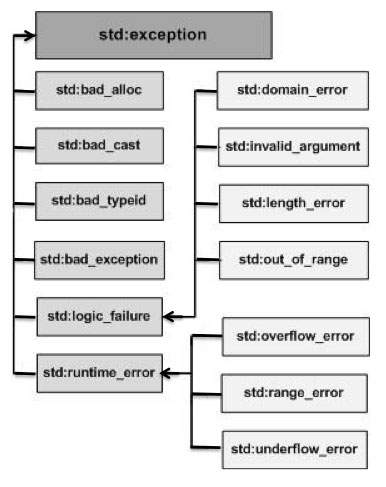
\includegraphics[height=0.55\paperheight]{imagens/cpp_exceptions.jpg}\\\tiny{Fonte: \url{https://www.tutorialspoint.com/cplusplus/images/cpp_exceptions.jpg}}
\end{figure}
\end{itemize}
\end{frame}

%-------------------------------------------------------
\begin{frame}\frametitle{Exceções Personalizadas}
\begin{itemize}
	\item É possível definir exceções personalizadas derivando a classe \texttt{exception} e eventualmente sobrescrevendo seus métodos
    \item O próximo exemplo mostra como usar a classe \texttt{exception} para implementar uma exceção personalizada
\end{itemize}
\end{frame}

%-------------------------------------------------------
\begin{frame}[fragile]\frametitle{Exemplo 3}
\lstinputlisting[basicstyle=\ttfamily\tiny]{src/exemplo03.cpp}
\end{frame}

%=======================================================
\section{Exercício}

%-------------------------------------------------------
\begin{frame}\frametitle{Exercício 1}
\begin{enumerate}
	\scriptsize
	\item Nas páginas a seguir você encontra a implementação de um Tipo Abstrato de Dados (TAD) para uma pilha de inteiros (arquivos \texttt{IntStack.hpp}, \texttt{IntStack.cpp} e \texttt{IntStackMain.cpp}). Esta classe (\texttt{IntStack}), possui os seguintes métodos em sua interface:\\
	\begin{itemize}
		\tiny
		\item \texttt{IntStack(int mxSz = 10)}: construtor que recebe o tamanho máximo da pilha
		\item \texttt{~IntStack()}: destrutor
		\item \texttt{int size()}: retorna o número de elementos da pilha
		\item \texttt{int maxSize()}: retorna o número máximo de elementos suportado pela pilha
		\item \texttt{bool isEmpty()}: retorna \texttt{true}, se a pilha estiver vazia, ou \texttt{false}, em caso contrário
		\item \texttt{bool isFull()}: retorna \texttt{true}, se a pilha estiver cheia, ou \texttt{false}, em caso contrário
		\item \texttt{void clear()}: esvazia a pilha
		\item \texttt{bool push(const int e)}: insere o elemento no topo da pilha (retorna \texttt{true}, em caso de sucesso, ou \texttt{false}, se NÃO houver espaço)
		\item \texttt{bool pop(int \&e)}: remove e retorna (por referência) o elemento do topo da pilha (retorna \texttt{true}, em caso de sucesso, ou \texttt{false}, a pilha estiver vazia)
		\item \texttt{bool top(\&e)}: retorna (por referência) o elemento do topo da pilha, mas não o remove da pilha (retorna \texttt{true}, em caso de sucesso, ou \texttt{false}, a pilha estiver vazia)
	\end{itemize}
	Modifique esta classe para que ela utilize \texttt{vector} da STL, \emph{templates} (de forma que ela NÃO fique restrita a inteiros) e exceções para os casos em que alguma operação inválida seja executada sobre a pilha. Com isso a interface dos seguintes métodos será alterada:\\
	\begin{itemize}
		\tiny
		\item \texttt{void push(T \&)}: insere o elemento no topo da pilha
		\item \texttt{T pop()}: remove e retorna o elemento do topo da pilha
		\item \texttt{T top() const}: retorna o elemento do topo da pilha, mas não o remove da pilha
	\end{itemize}
\end{enumerate}
\end{frame}


%-------------------------------------------------------
\begin{frame}\frametitle{Exemplo de Implementação: \texttt{IntStack.hpp}}
\lstinputlisting[basicstyle=\ttfamily\tiny]{src/IntStack.hpp}
\end{frame}

%-------------------------------------------------------
\begin{frame}\frametitle{Exemplo de Implementação: \texttt{IntStack.cpp}}
\fontsize{3pt}{5pt}\selectfont{
\lstinputlisting{src/IntStack.cpp}
}
\end{frame}

%-------------------------------------------------------
\begin{frame}\frametitle{Exemplo de Implementação: \texttt{IntStackMain.cpp}}
\fontsize{5pt}{6pt}\selectfont{
\lstinputlisting{src/IntStackMain.cpp}
}
\end{frame}

%-------------------------------------------------------
\end{document}

